\section{Fault Modeling with the Safety Annex: Methodology}
\label{sec:fault_modeling}

To demonstrate the fault modeling capabilities of the Safety Annex we will use the \gls{wbs} described in \gls{air} 6110~\cite{AIR6110}.  This system is a well-known example that has been used as a case study for safety analysis, formal verification, and contract based design~\cite{DBLP:conf/cav/BozzanoCPJKPRT15, 10.1007/978-3-319-11936-6-7, CAV2015:BoCiGrMa, Joshi05:SafeComp}. This section first describes the \gls{wbs} system and then uses that system description to illustrate fault modeling using \gls{aadl}, \gls{agree}, and the safety annex. The analysis results of this examples will be described in Section~\ref{sec:fault_analysis_2}.

\subsection{Wheel Brake System Overview}
The preliminary work for the safety annex was based on a simple model of the \gls{wbs}~\cite{Stewart17:IMBSA}. To demonstrate a more complex fault modeling process, we constructed a functionally and structurally equivalent \gls{aadl} version of the more complex \gls{wbs} which was captured in NuSMV/xSAP models~\cite{DBLP:conf/cav/BozzanoCPJKPRT15}. Figure~\ref{fig:wbs} shows only one pair of wheels and their interactions with the rest of the system for clarity. The full version that was modeled in \gls{aadl} contains a total of 8 wheels.

\begin{figure}[h!]
	\centering
	%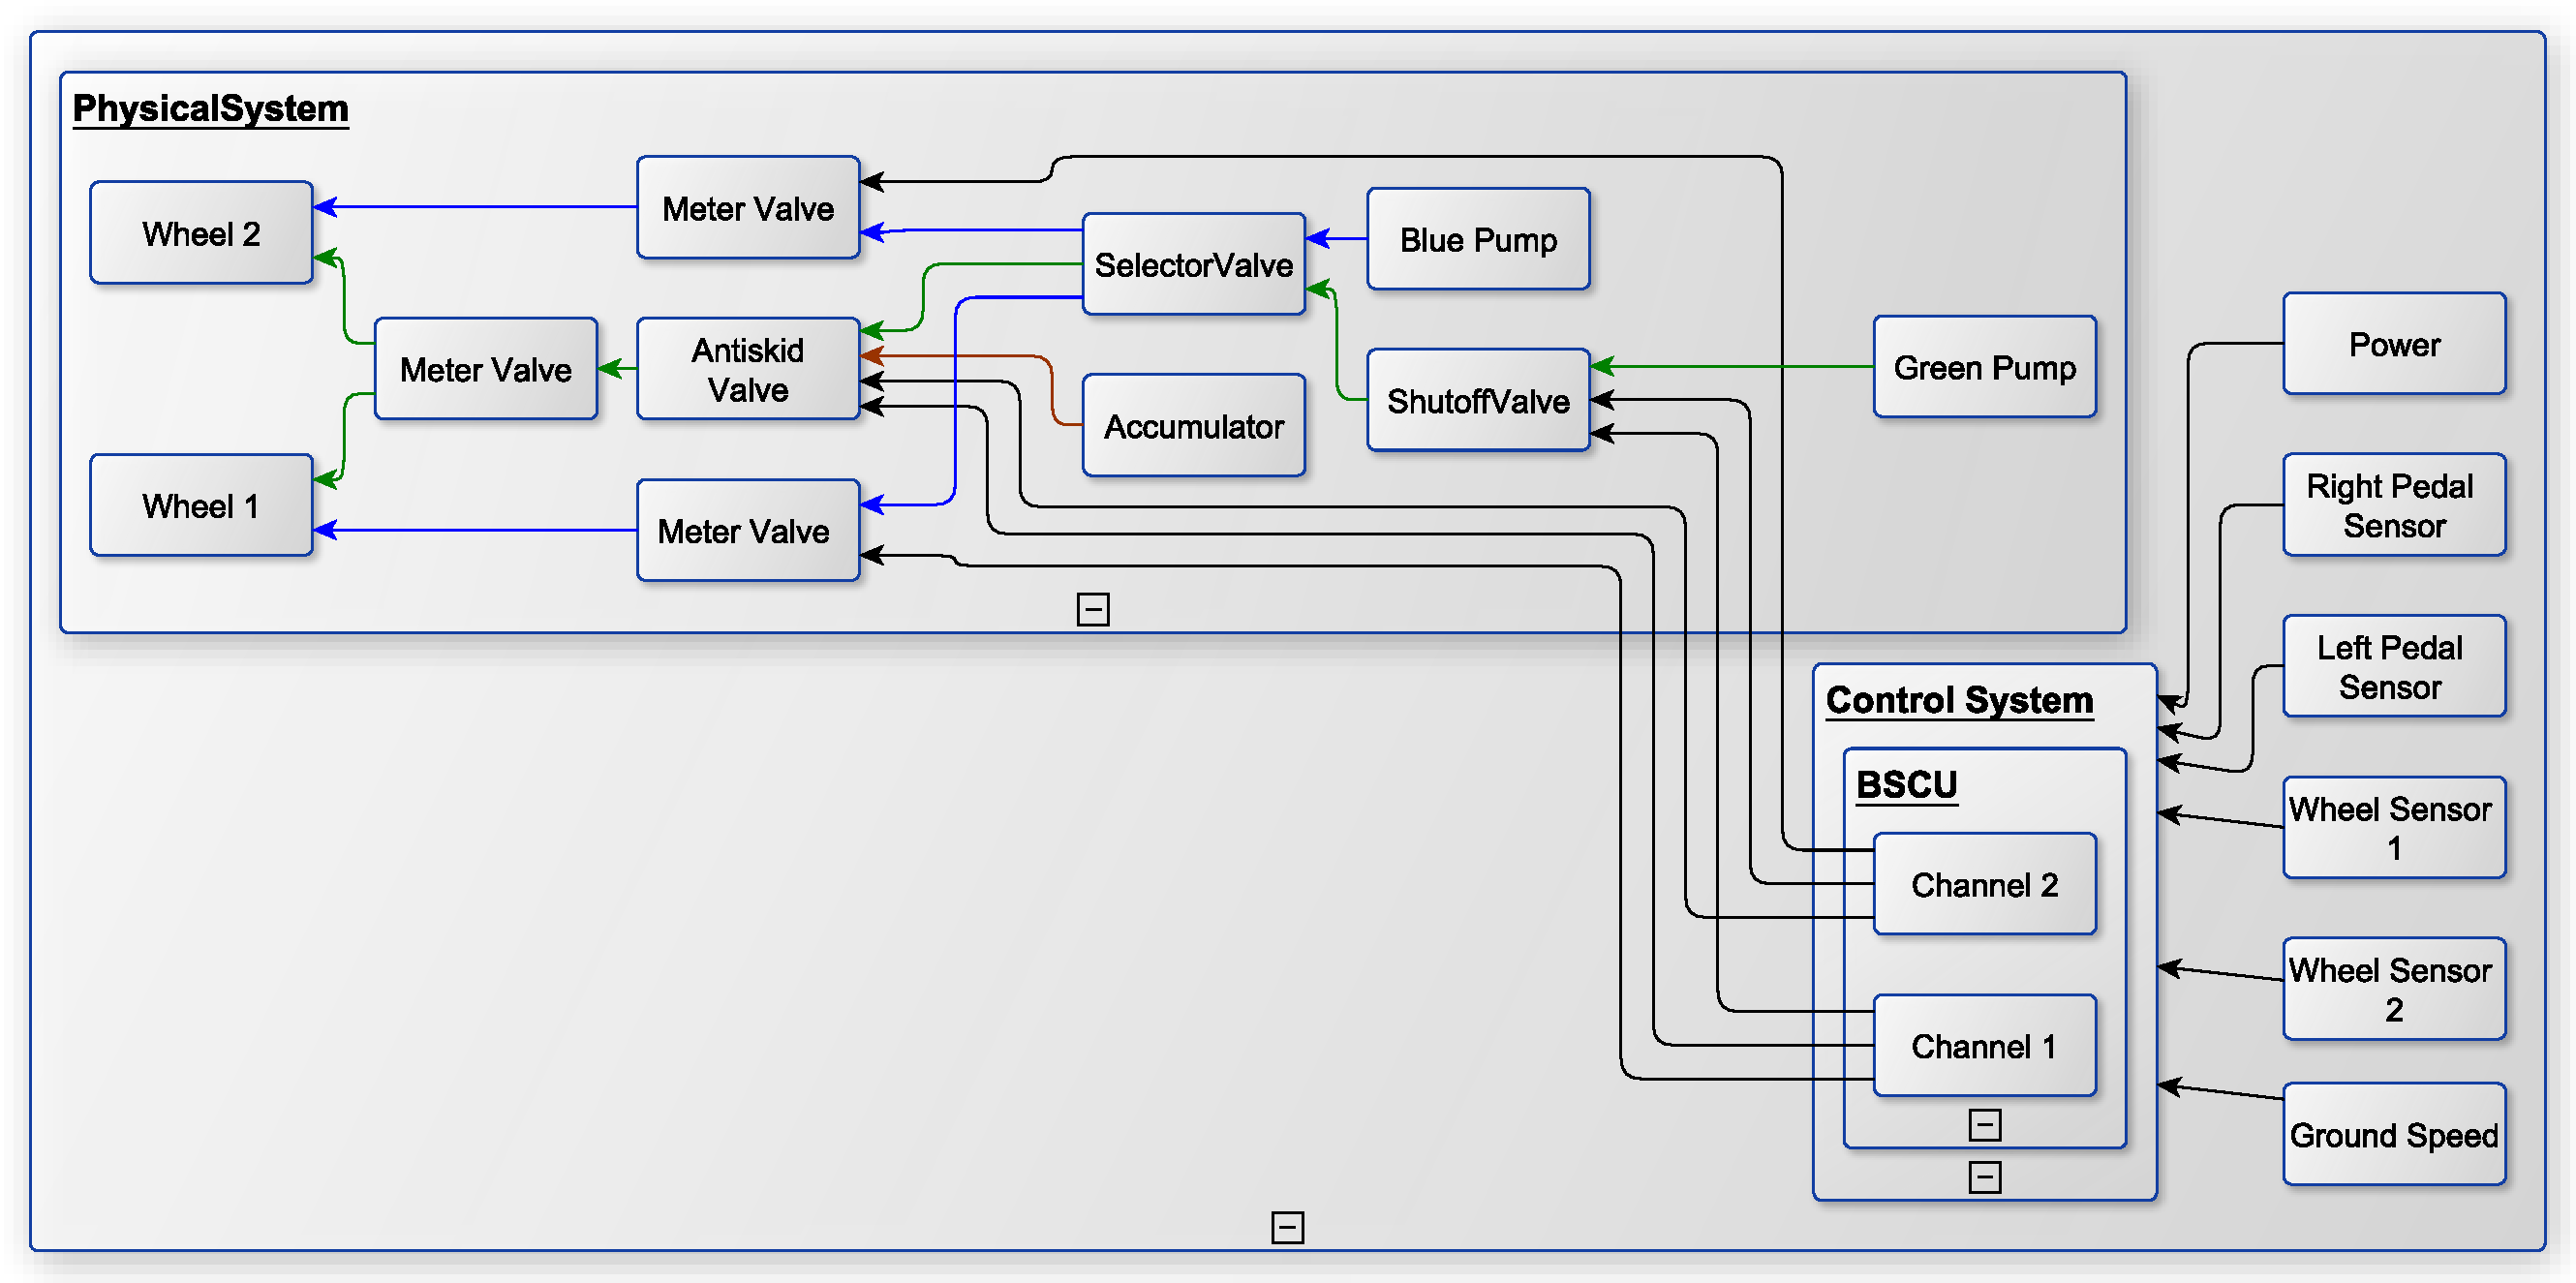
\includegraphics[trim=0 9 0 5,clip,width=\textwidth]{images/wbs_arch4_diagram.pdf}
	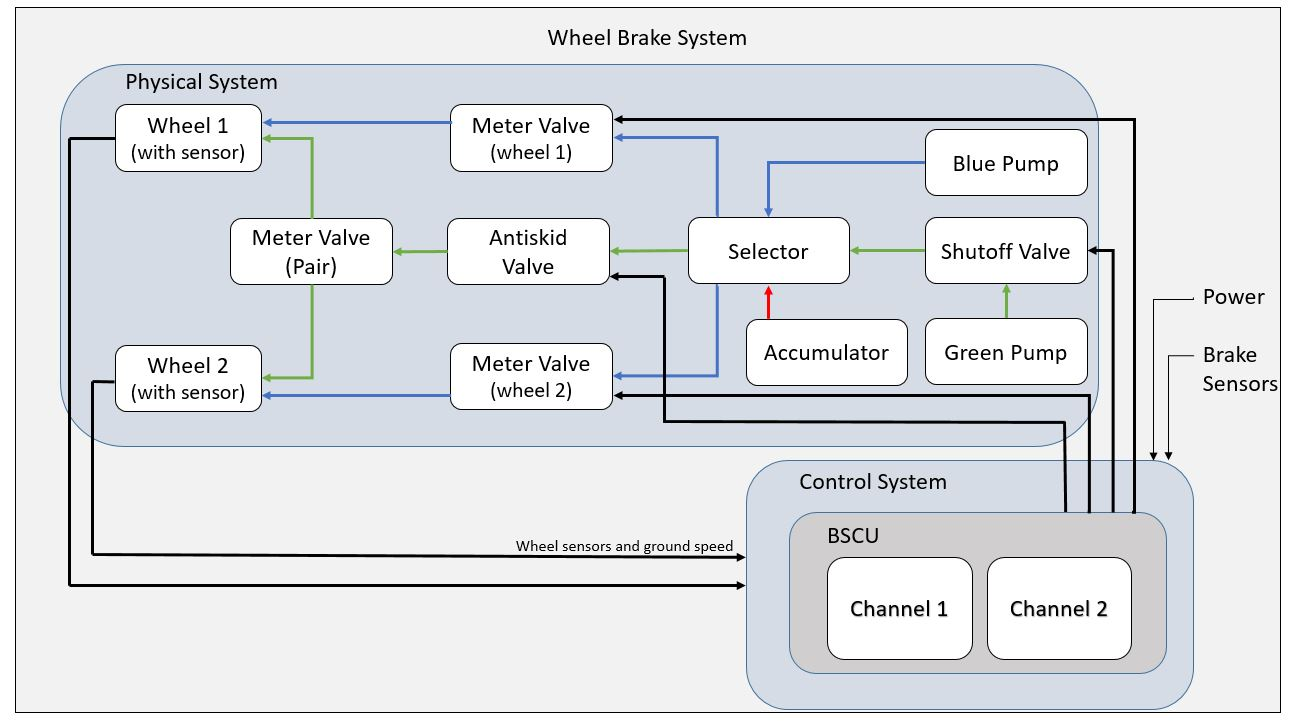
\includegraphics[width=\textwidth]{images/wbs_arch4.jpg}
	\caption{A Two-Wheel Diagram of the Wheel Brake System}
	\label{fig:wbs}
\end{figure} 

The \gls{wbs} is composed of two main parts: the control system and the electro-mechanical physical system. The physical system consists of redundant hydraulic circuits (designated green and blue) running from hydraulic pumps to wheel brakes as well as valves that control the hydraulic fluid flow. The physical system provides braking force to each of the eight wheels of the aircraft. The wheels are all mechanically braked in pairs. The control system commands electronic control of the physical system. %The \gls{bscu} of the control system electronically commands the physical system. 
The \gls{bscu} consists of two channels for redundancy in case a detectable fault occurs in the active channel. The \gls{bscu} also commands antiskid braking and controls the operating mode of the system through commands to the selector valve. These commands are sent to a selector valve component which selects which hydraulic pump supplies pressure depending on which operating mode the system is currently in. 

Top level inputs to the system include the mechanical pedal sensors and the power. These are considered black box components. The only pilot interaction modeled in this system is through mechanical braking command.

There are three operating modes in the WBS model:

\begin{itemize}
	\renewcommand{\labelitemi}{\textbullet}
	\item In \textit{normal} mode, the system uses the green hydraulic pump and one meter valve per each of the eight wheels (in Figure~\ref{fig:wbs}, this corresponds to e.g., ''Meter Valve (wheel 1)". Each of the meter valves are controlled through electronic commands coming from the active channel of the \gls{bscu}. These signals provide braking and antiskid commands for each wheel. The braking command is determined through a sensor on the pedal and the antiskid command is determined by the wheel sensors and detection of skid. 
	\item In \textit{alternate} mode, the system uses the blue hydraulic pump, four meter valves (one per wheel pair as shown in Figure~\ref{fig:wbs}: ''Meter Valve (Pair)"), and four antiskid shutoff valves (one per wheel pair). The meter valves are mechanically commanded through the pilot pedal corresponding to each wheel pair. If the selector detects lack of pressure in the green circuit, it switches to the blue circuit. Alternatively, if the \gls{bscu} detects a fault in the normal (green) mode of operation, the \gls{bscu} may likewise shut off the green pump and force a switch to alternate (blue) mode of operation. 
	\item \textit{Emergency} mode is triggered when the blue hydraulic pump fails. The accumulator component has a reserve of pressurized hydraulic fluid and will supply this to the blue circuit in emergency mode. 
\end{itemize}

The \gls{wbs} architecture model in \gls{aadl} contains 30 different kinds of components, 169 component instances, and a model depth of 5 hierarchical levels. 

\subsection{Nominal Model} 
The nominal, or behavioral, model is encoded using the \gls{agree} annex and the behavior is based on descriptions found in \gls{air}6110. The top level system properties are given by the requirements and safety objectives in \gls{air}6110. All of the subcomponent contracts support these system safety objectives through the use of assumptions on component input and guarantees on the output. The \gls{wbs} behavioral model in the \gls{agree} annex includes one top-level assumption and  11 top-level system properties, with 113 guarantees allocated to subsystems.  

An example system safety property is to ensure that there is no inadvertent braking of any of the wheels. This is based on a failure condition described in \gls{air}6110: \textit{Inadvertent wheel braking on one wheel during takeoff shall be less than 1E-9 per takeoff}. 
Inadvertent braking means that braking force is applied at the wheel but the pilot has not pressed the brake pedal.  In addition, the inadvertent braking requires that power and hydraulic pressure are both present, the plane is not stopped, and the wheel is rolling (not skidding). The property is stated in \gls{agree} such that inadvertent braking does \textit{not} occur, as shown in Figure \ref{fig:inadvertent_braking}. (The expression shown in Figure~\ref{fig:inadvertent_braking} \textit{true $\rightarrow$ property} in \gls{agree} is true in the initial state and then afterwards it is only true if property holds.)

\begin{figure}[h!]
	%\vspace{-0.2in}
	\begin{center}
		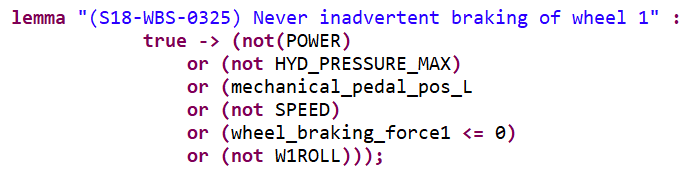
\includegraphics[width=.7\textwidth]{images/inadvertent_braking.png}
	\end{center}
	\vspace{-0.3in}
	\caption{AGREE Contract for Top Level Property: Inadvertent Braking}
	\label{fig:inadvertent_braking}
	%\vspace{-0.2in}
\end{figure}

%%%%%%%%%%%%							COMPONENT FAULT MODELING
\subsection{Component Fault Modeling}
\label{subsec:compFM}
The usage of the terms error, failure, and fault are defined in \gls{arp}4754A and are described here for ease of understanding~\cite{SAE:ARP4754A}. An \textit{error} is a mistake made in implementation, design, or requirements. A \textit{fault} is the manifestation of an error and a \textit{failure} is an event that occurs when the delivered service of a system deviates from correct behavior. If a fault is activated under the right circumstances, that fault can lead to a failure. The terminology used in EMV2 differs slightly for an error: an \textit{error} is a corrupted state caused by a \textit{fault}. The error propagates through a system and can  manifest as a \textit{failure}. In this report, we use the \gls{arp}4754A terminology with the added definition of \textit{error propagation} as used in EMV2. An \textit{error} is a mistake made in design or code and an \textit{error propagation} is the propagation of the corrupted state caused by an active \textit{fault}. 

The Safety Annex is used to add potential faulty behaviors to a component model. Within the \gls{aadl} component instance model, an annex is added which contain the fault definitions for the given component. The flexibility of the fault definitions allows the user to define numerous types of fault \textit{nodes} by utilizing the \gls{agree} node syntax. A library of common fault nodes has been written and is available in the project GitHub repository~\cite{SAGithub}. Examples of such faults include valves being stuck open or closed, output of a software component being nondeterministic, or power being cut off.  When the fault analysis requires fault definitions that are more complex, these nodes can easily be written and used in the model. 

When a fault is activated by its specified triggering conditions, it modifies the output of the component. This faulty behavior may lead to a violation of the contracts of other components in the system, including assumptions of downstream components. The impact of a fault is computed by the \gls{agree} model checker when the safety analysis is run on the fault model. 

As an illustration of fault modeling using the Safety Annex, we look at one of the components important to the inadvertent braking property: the brake pedal. When the mechanical pedal is pressed, a sensor reads this information and passes an electronic signal to the \gls{bscu} which then commands hydraulic pressure to the wheels. 

Figure~\ref{fig:sensor} shows the \gls{aadl} pedal sensor component with a contract for its nominal behavior. (The expression \textit{true $\rightarrow$ property} in \gls{agree} is true in the initial state and then afterwards it is only true if property holds.) The sensor has only one input, the mechanical pedal position, and one output, the electrical pedal position. 
A property that governs the behavior of the component is that the mechanical position should always equal the electronic position. 

\begin{figure}[h!]
	\hspace*{-2cm}
	%\vspace{-0.55in} 
	\begin{center}
		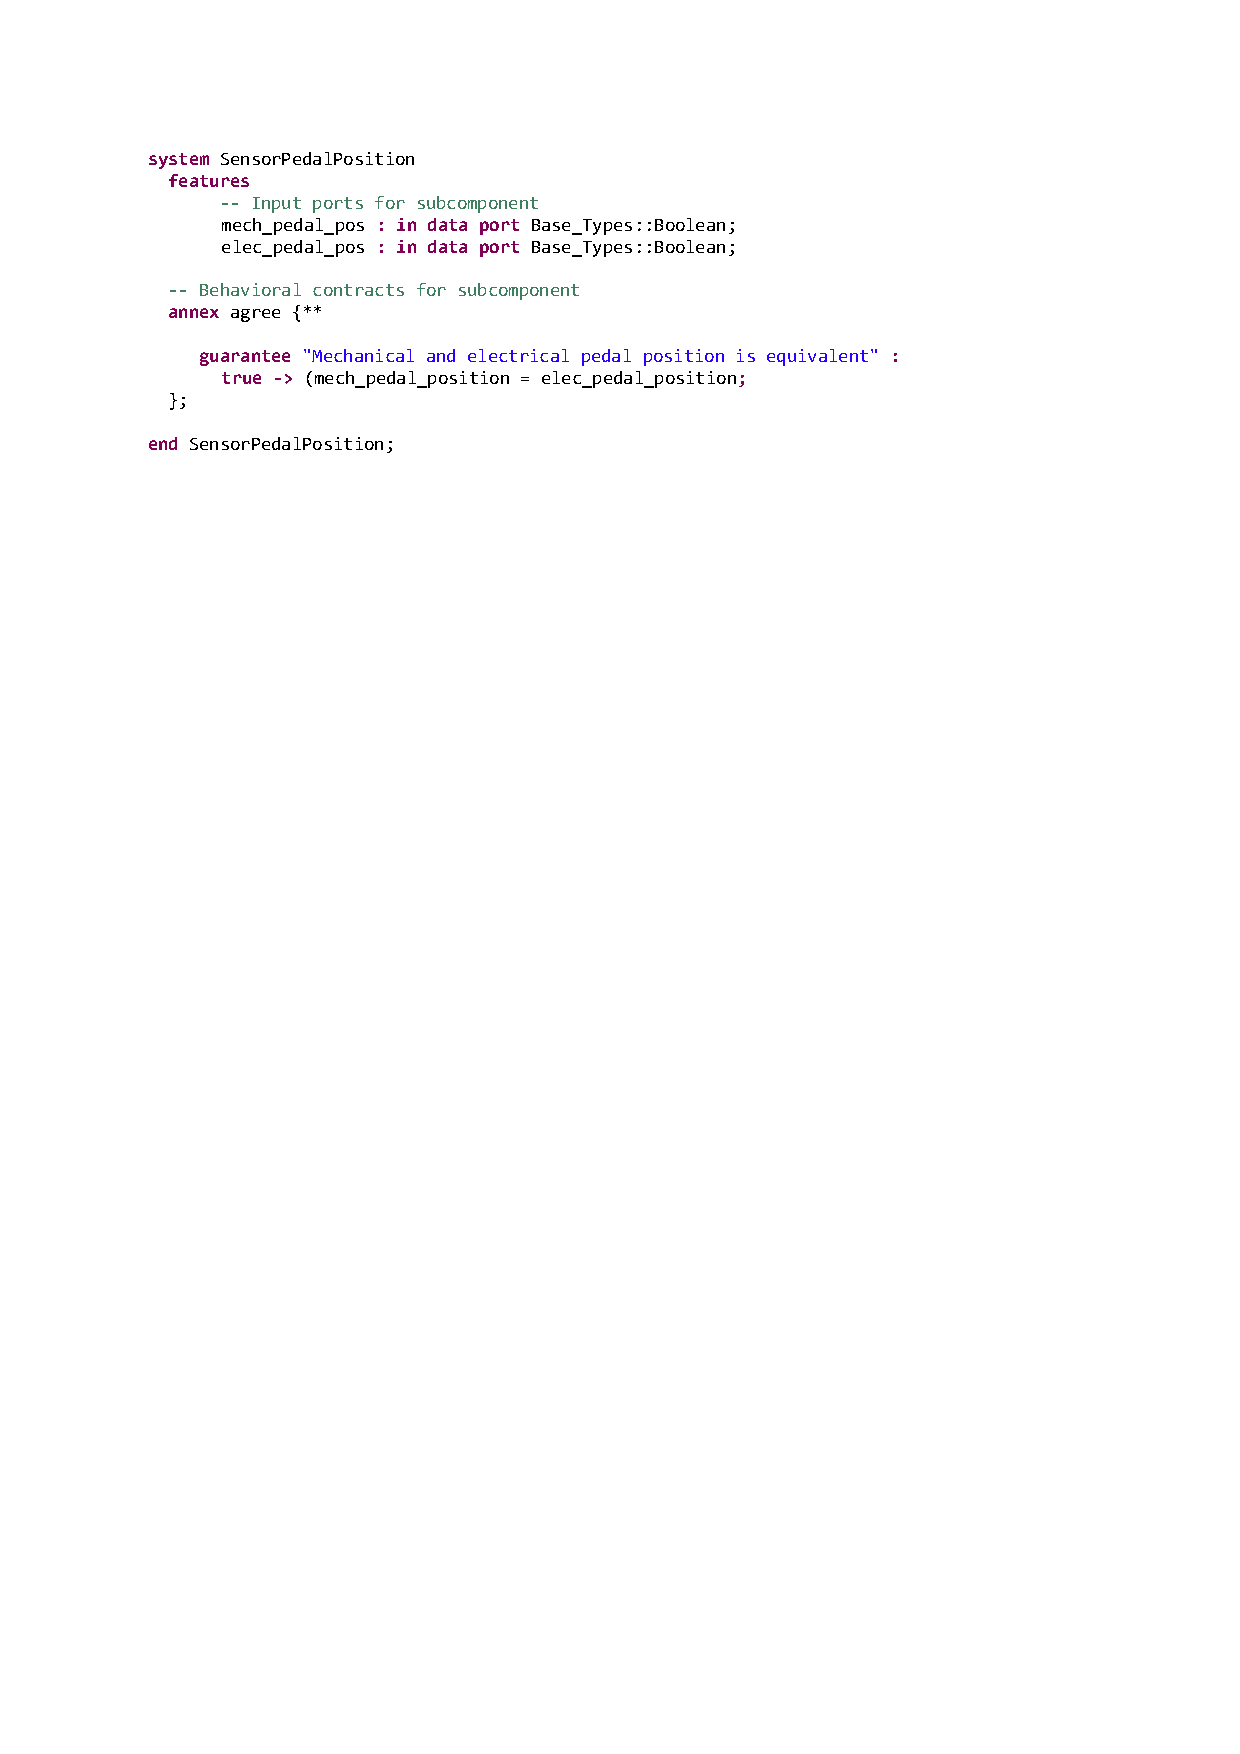
\includegraphics[trim=0 640 -10 70,clip,width=1.5\dimexpr\textwidth-2cm\relax]{images/system_sensor.pdf}
		\vspace{-0.3in}
		\caption{An AADL System Type: The Pedal Sensor}
		\label{fig:sensor}
	\end{center}
	\vspace{-0.2in}
\end{figure}

One possible failure for the pedal sensor is inversion of its output value. This fault can be triggered with probability $5.0\times 10^{-6}$ as described in \gls{air}6110 (in practice, the component failure probability is 
collected from hardware specification sheets).  
The Safety Annex definition for this fault is shown in Figure~\ref{fig:sensorFault}. Fault behavior is defined through the use of a fault node called \textit{inverted\_fail}.  When the fault is triggered, the nominal output of the component (\textit{elec\_pedal\_position}) is replaced with its failure value (\textit{val\_out}). 

\begin{figure}[h!]
	\hspace*{-2cm}
	%\vspace{-0.5in} 
	\begin{center}
		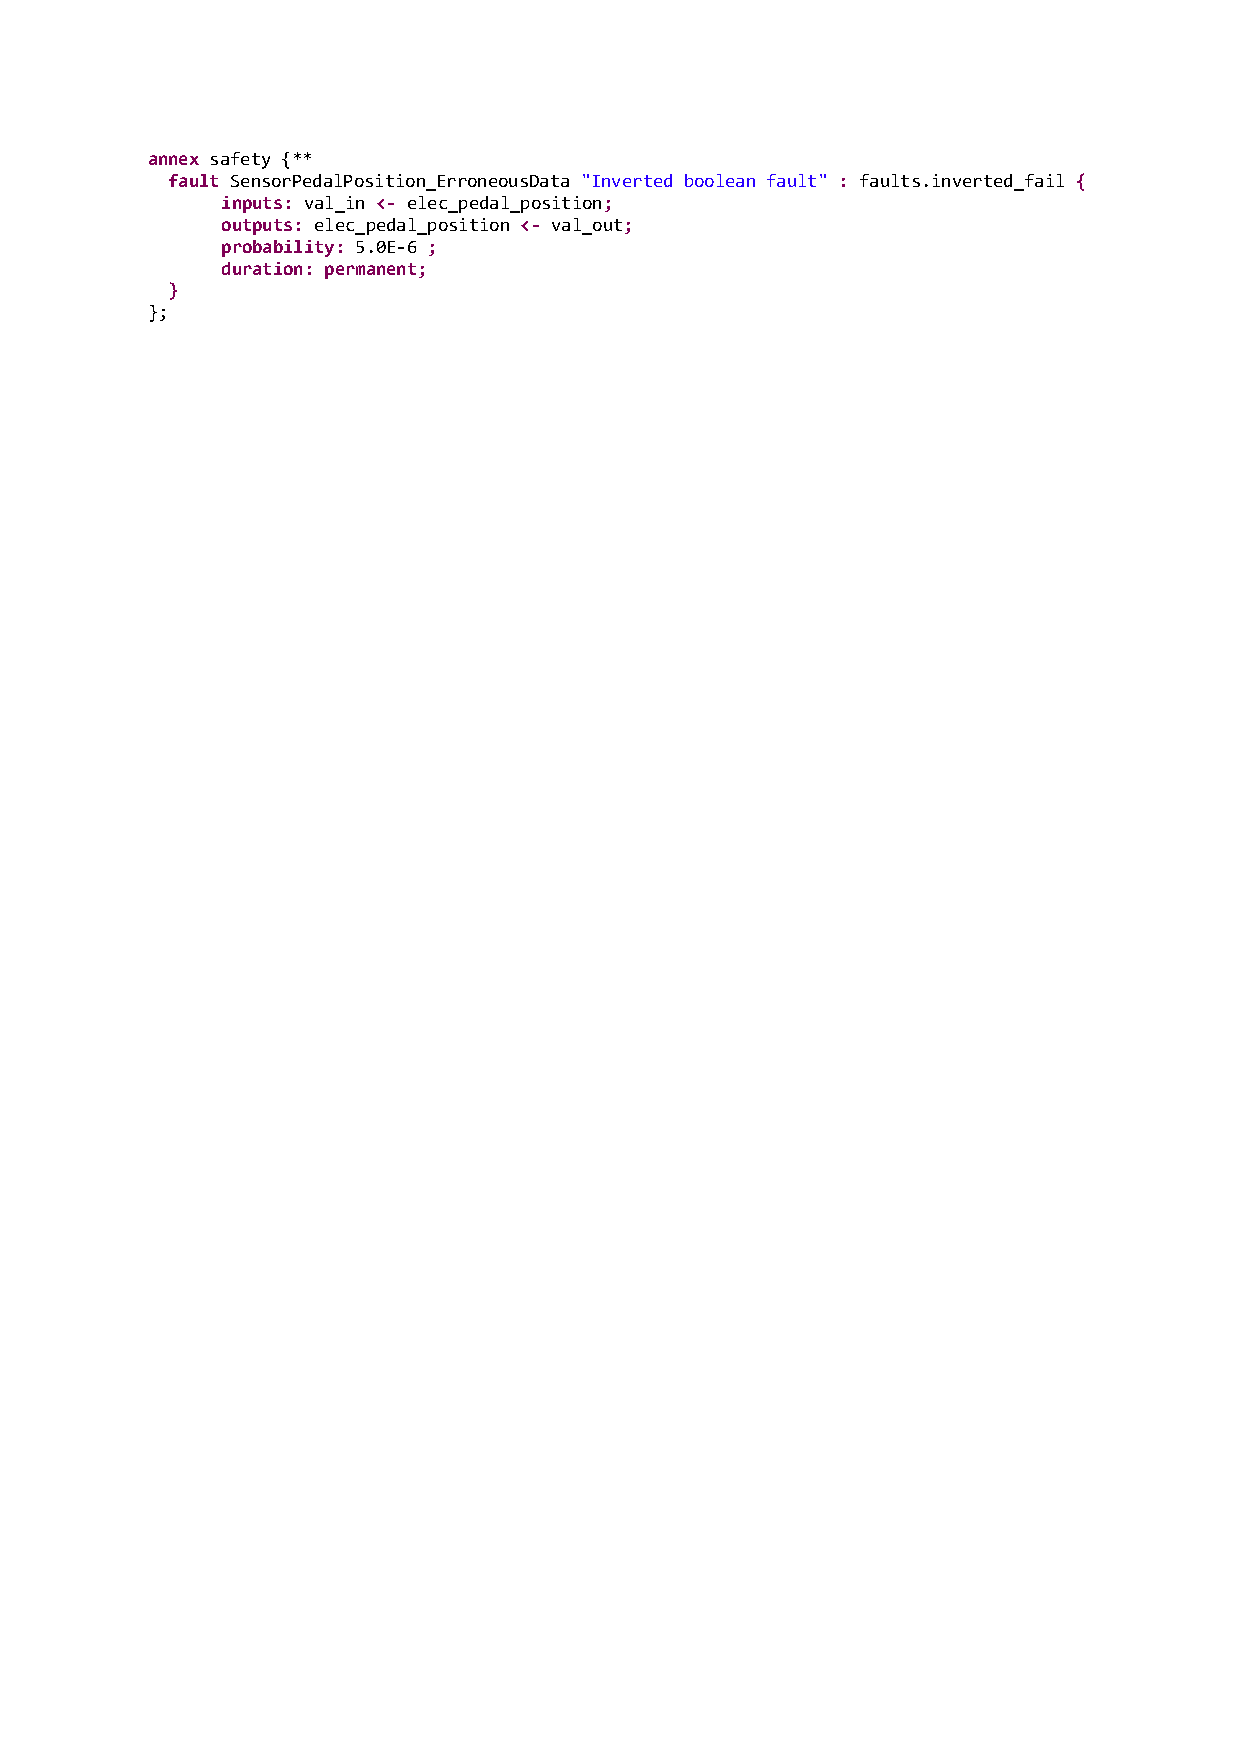
\includegraphics[trim=0 680 -10 70,clip,width=1.5\dimexpr\textwidth-2cm\relax]{images/safetyannex_sensorfault.pdf}
		\vspace{-0.2in}
		\caption{The Safety Annex for the Pedal Sensor}
		\label{fig:sensorFault}
	\end{center}
	\vspace{-0.2in}
\end{figure}

The \gls{wbs} fault model expressed in the Safety Annex contains a total of 33 fault definitions and 141 fault instances. The large number of fault instances is due to the redundancy in the system design and its replication to control 8 wheels.

%%%%%%%%%%%								IMPLICIT ERROR PROPAGATION
\subsection{Implicit Error Propagation}
\label{subsec:implicit}
In the Safety Annex approach, faults are captured as faulty behaviors that augment the system behavioral model in AGREE contracts. No explicit error propagation is necessary since the faulty behavior propagates through the nominal behavior contracts in the system model just as in the real system. The effects of any triggered fault are manifested through analysis of the \gls{agree} contracts. 

By contrast, in the \gls{aadl} Error Model Annex, Version 2 (EMV2)~\cite{EMV2} approach, all errors must be explicitly propagated through each component (by applying fault types on each of the output ports) for a component to have an impact on the rest of the system. To illustrate the key differences between implicit error propagation provided in the Safety Annex and the explicit error propagation provided in EMV2, we use a simplified behavioral flow from the WBS example using code fragments from EMV2, \gls{agree}, and the Safety Annex (Figure~\ref{fig:comparison_with_EMV2}). 

\begin{figure}[t]
	%\hspace*{-2cm}
	\vspace{-0.19in}
	\centering
	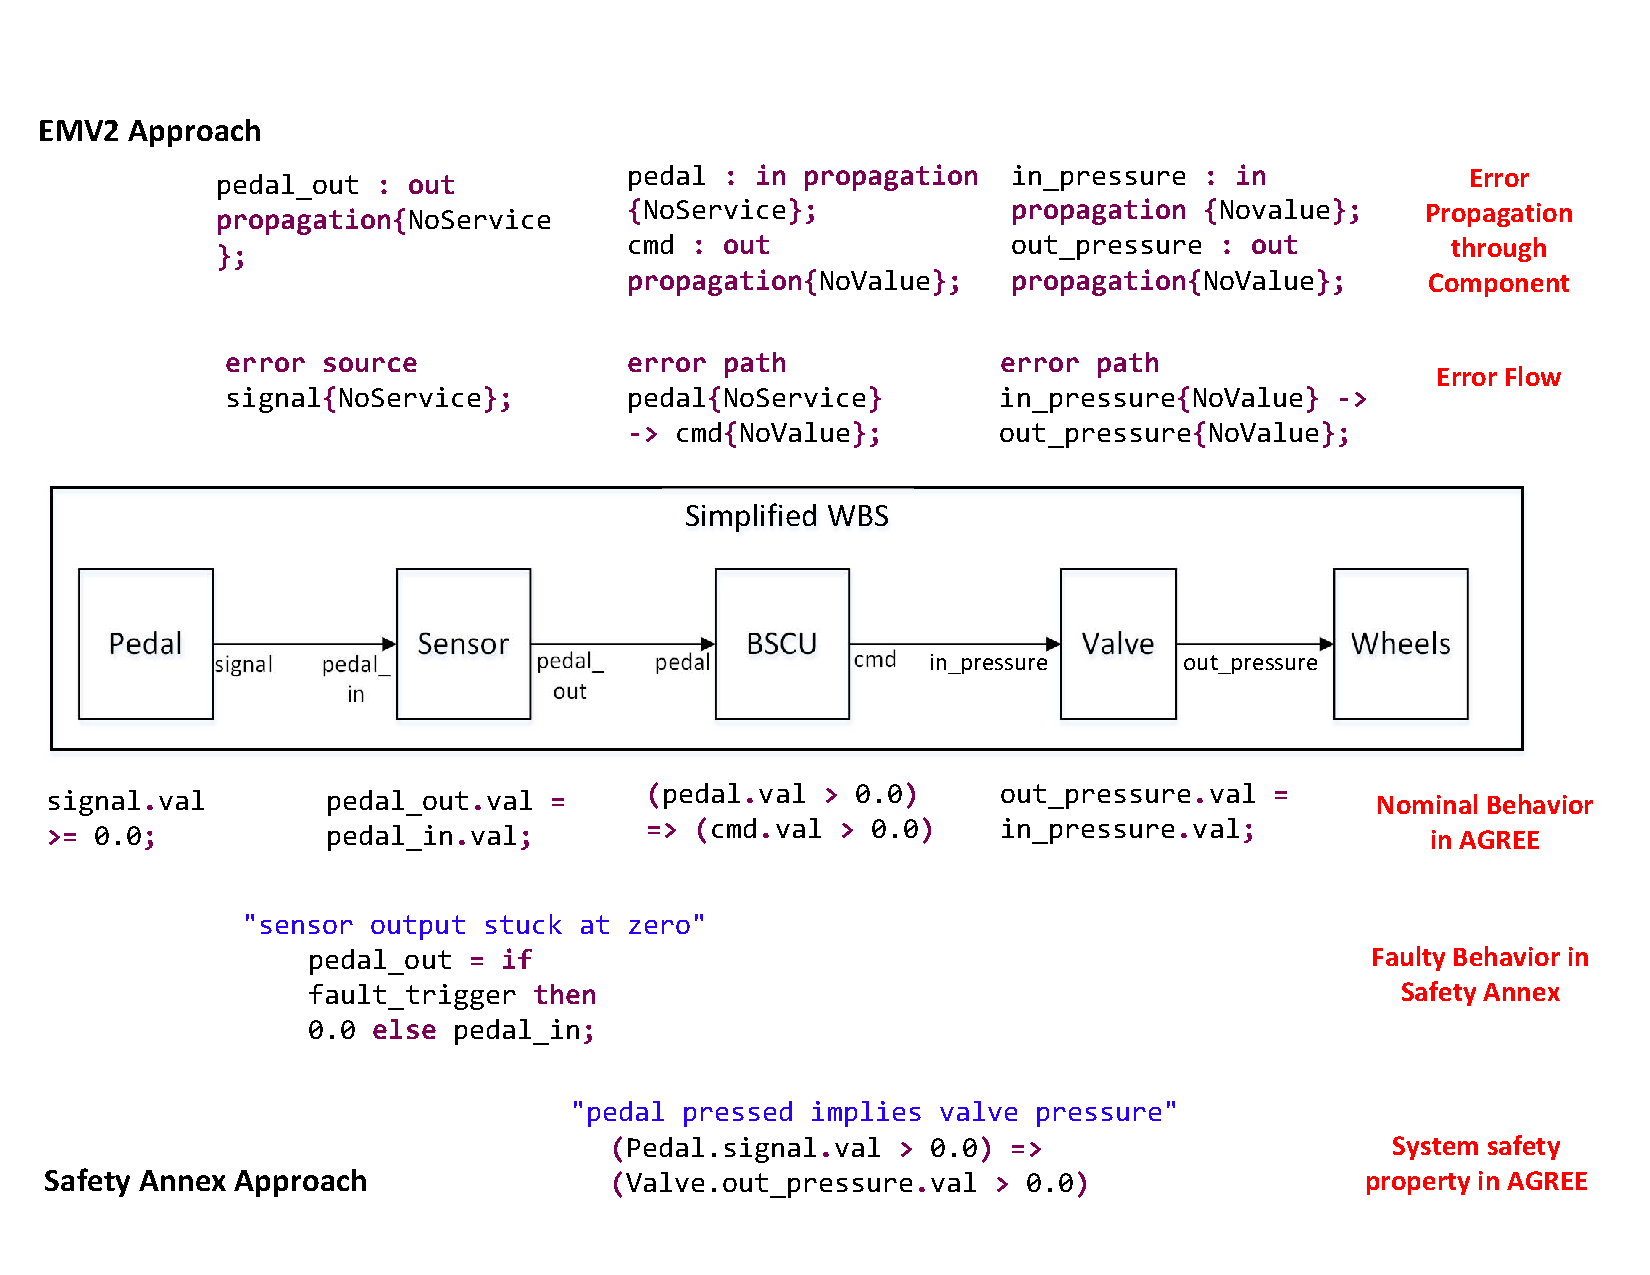
\includegraphics[trim=0 9 0 5,clip,width=\textwidth]{images/Comparison_with_EMV2.pdf}
	%\vspace{-0.3in}
	\caption{Differences between Safety Annex and EMV2}
	\label{fig:comparison_with_EMV2}
	%\vspace{-0.2in}
\end{figure} 

In this simplified \gls{wbs} system, the physical signal from the pedal component is detected by the sensor and the pedal position value is passed to the \gls{bscu} components.  The \gls{bscu} generates a pressure command to the valve component which applies hydraulic brake pressure to the wheels. 

In the EMV2 approach (top half of Figure~\ref{fig:comparison_with_EMV2}), the ``NoService'' fault is explicitly propagated through all of the components. These fault types are essentially tokens rather than a specifiction of the faulty behavior. At the system level, analysis tools supporting the EMV2 annex can aggregate the propagation information from different components to compose an overall fault flow diagram or fault tree. 

When a fault is triggered in the Safety Annex (bottom half of Figure~\ref{fig:comparison_with_EMV2}), the output behavior of the sensor component is modified. In this case the result is a ``stuck at zero'' error. The behavior of the \gls{bscu} receives a zero input signal and responds as if the pedal has not been pressed. This will cause the top level system contract to fail: {\em pedal pressed implies brake pressure output is positive}.

%%%%%%%%%%%%%%%								EXPLICIT ERROR PROPAGATION
\subsection{Explicit Error Propagation} 
\label{subsec:explicit}
Failures in \gls{hw} components can trigger behavioral faults in the system components that depend on them. For example, a \gls{cpu} failure may trigger faulty behavior in the threads bound to that \gls{cpu}. In addition, a failure in one \gls{hw} component may trigger failure in other \gls{hw} components located nearby, such as overheating, fire, or explosion
in the containment location. 
The Safety Annex provides the capability to explicitly model the impact of hardware failures on other faults, whether dependent or independent. The explicit propagation to non behavioral faults is similar to that provided in EMV2.

To better model faults at the system level that are dependent on \gls{hw} failures, a fault model element is introduced called a \textit{hardware fault}. Users are not required to specify behavioral effects for the \gls{hw} faults, nor are data ports necessary on which to apply the fault definition. An example of a model component fault declaration is shown below:
\begin{figure}[h!]
	\vspace{-0.1in}
	\begin{center}
	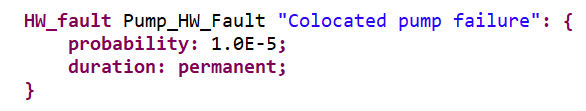
\includegraphics[width=.6\textwidth]{images/hw_fault2.png}
	\end{center}
	\vspace{-0.3in}
	\caption{Hardware Fault Definition}
	\label{fig:hwFault}
	%\vspace{-0.2in}
	\vspace{-0.2in}
\end{figure}

Users specify dependencies between the \gls{hw} component faults and faults that are defined in other components, either \gls{hw} or \gls{sw}. The hardware fault then acts as a trigger for dependent faults. This allows a simple propagation from the faulty \gls{sw} component to the \gls{sw} components that rely on it, affecting the behavior on the outputs of the affected \gls{sw} components.

In the \gls{wbs} example, assume that both the green and blue hydraulic pumps are located in the same compartment in the aircraft and an explosion in this compartment rendered both pumps inoperable. The \gls{hw} fault definition can be modeled first in the green hydraulic pump component as shown in Figure~\ref{fig:hwFault}. The activation of this fault triggers the activation of related faults as seen in the \textit{propagate\_to} statement shown in Figure~\ref{fig:hwFaultProp}. Notice that these pumps need not be connected through a data port in order to specify this propagation. 

\begin{figure}[h!]
	\vspace{-0.1in}
	\begin{center}
		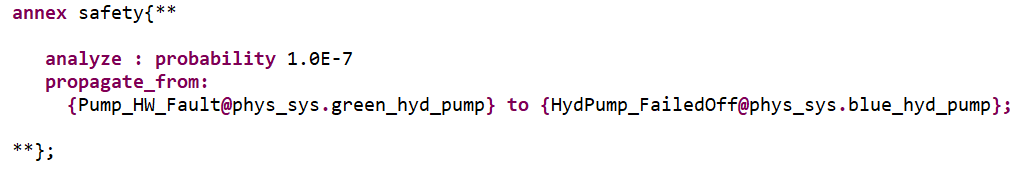
\includegraphics[width=1.0\textwidth]{images/hw_prop_stmt.png}
	\end{center}
	\vspace{-0.3in}
	\caption{Hardware Fault Propagation Statement}
	\label{fig:hwFaultProp}
	%\vspace{-0.2in}
	%\vspace{-0.1in}
\end{figure}

The fault dependencies are specified in the system implementation where the system configuration that causes the dependencies becomes clear (e.g., binding between \gls{sw} and \gls{hw} components, co-location of \gls{hw} components). 


%%%%%%%%%%%%%								FAULT ANALYSIS STMTS
\subsection{Fault Analysis Statements}
\label{subsec:analysisStmts}
The fault analysis statement (also referred to as the fault hypothesis) resides in the \gls{aadl} system implementation that is selected for verification. This may specify the maximum number of faults that can be active at any point in execution (Figure~\ref{fig:hypothesisMaxN}).

\begin{figure}[h!]
	\vspace{-0.1in}
	\begin{center}
		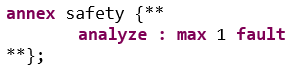
\includegraphics[width=0.4\textwidth]{images/hypothesisMaxN.png}
	\end{center}
	\vspace{-0.1in}
	\caption{Max N Faults Analysis Statement}
	\label{fig:hypothesisMaxN}
\end{figure}
Alternatively, the fault analsis statement may specify that the only faults to be considered are those whose probability of simultaneous occurrence is above some probability threshold (Figure~\ref{fig:hypothesisProb}). 

\begin{figure}[h!]
	\vspace{-0.1in}
	\begin{center}
		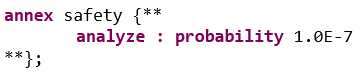
\includegraphics[width=0.5\textwidth]{images/hypothesisProb.png}
	\end{center}
	\vspace{-0.1in}
	\caption{Probability Analysis Statement}
	\label{fig:hypothesisProb}
\end{figure}

Tying back to the fault tree analysis in traditional safety analysis, the former is analogous to restricting the cutsets to a specified maximum number of terms, and the latter is analogous to restricting the cutsets to only those whose simultaneous probability is above some set value. In the former case, we assert that the sum of the true {\em fault\_\_trigger} variables is at or below some integer threshold.  In the latter, we determine all combinations of faults whose probabilities are above the specified probability threshold, and describe this as a proposition over {\em fault\_\_trigger} variables. 

With the introduction of dependent faults, active faults are divided into two categories: independently active (activated by its own triggering event) and dependently active (activated when the faults they depend on become active). The top level fault hypothesis applies to independently active faults. Faulty behaviors augment nominal behaviors whenever their corresponding faults are active (either independently active or dependently active).

%%%%%%%%%%%%%%%%% 							ASYM FAULTS
\subsection{Asymmetric Faults and Implementation}
A \textit{Byzantine} or \textit{asymmetric} fault is a fault that presents different symptoms to different observers~\cite{Driscoll-Byzantine-Fault}. 
%In our modeling environment, asymmetric faults may be associated with a 
Consider a source component with an output that is connected to multiple inputs on different destination components. In this configuration, a \textit{symmetric} fault will result in all destination components observing the same faulty value from the source component. In an {\em asymmetric} fault, the destination components may observe different values from the source.  To capture the behavior of asymmetric faults %(``different symptoms to different observers''), 
it was necessary to extend our fault modeling mechanism in \gls{aadl}. 

To illustrate our implementation of asymmetric faults, assume a source component A has a 1-to-many output connected to four destination components (B-E) as shown in Figure~\ref{fig:commNodes} under ``Nominal System.'' If a symmetric fault was present on this output, all four connected components would see the same faulty behavior. An asymmetric fault should be able to present arbitrarily different values to the connected components. 

To this end, ``communication nodes'' are automatically inserted on each connection from component A to components B, C, D, and E (shown in Figure~\ref{fig:commNodes} under ``Fault Model Architecture''). From the users perspective, the asymmetric fault definition is associated with component A's output and the architecture of the model is unchanged from the nominal model architecture. Behind the scenes, these communication nodes are created to facilitate potentially different fault activations on each of these connections. The fault definition used on the output of component A will be inserted into each of these communication nodes as shown by the red circles at the communication node output in Figure~\ref{fig:commNodes}.
\begin{figure}[!htb]
        \center{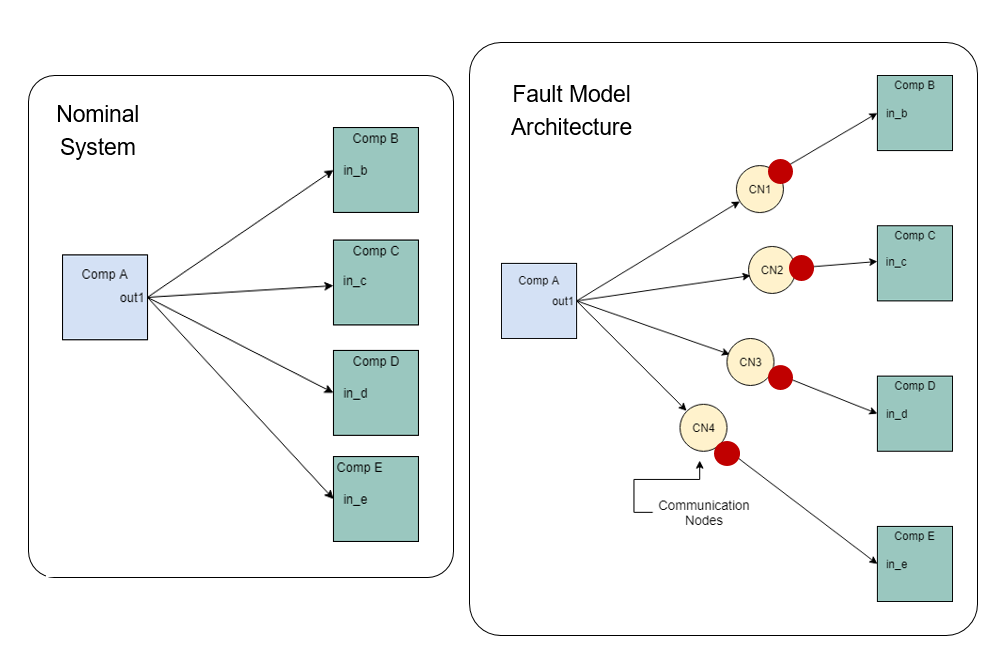
\includegraphics[width=0.8\textwidth] {images/commNodes.png}}
        \caption{\label{fig:commNodes} Communication Nodes in Asymmetric Fault Implementation}
\end{figure}

\begin{figure}[!htb]
        \center{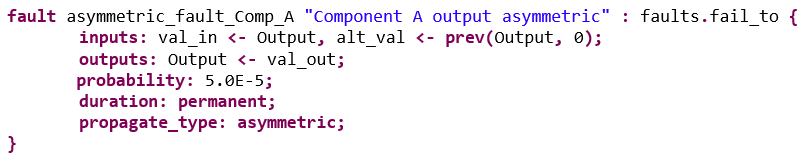
\includegraphics[width=\textwidth] {images/asymFaultDef.png}}
        \caption{\label{fig:asymFaultDef} Asymmetric Fault Definition in the Safety Annex}
\end{figure}

An asymmetric fault is defined for component A as in Figure~\ref{fig:asymFaultDef}. This fault defines an asymmetric failure on component A that when active, is stuck at a previous value (\textit{prev(Output, 0)}). This can be interpreted as the following: some connected components may only see the previous value of component A output and others may see the correct (current) value when the fault is active. This fault definition is injected into the communication nodes and which of the connected components see an incorrect value is completely nondeterministic. Any number of the communication node faults (0…all) may be triggered upon activation of the main asymmetric fault on the source output.



